\documentclass[12pt]{article}
\usepackage[margin=2cm]{geometry} 
\usepackage{titling}
\usepackage{graphicx}
\usepackage{float}
\usepackage[hidelinks]{hyperref}
\usepackage[italian]{babel}
\usepackage{subcaption}

\setlength\parindent{0pt}
\setlength{\parskip}{1em}
\setlength{\droptitle}{-2cm}

\title{Istruzioni d'uso AR Sandbox (ad uso interno)}
\author{Università della Svizzera italiana}
\date{Versione \today}


\begin{document}
\maketitle
\tableofcontents
\newpage


\section{Installazione}\label{installation}

\subsection{Componenti}

\begin{itemize}
	\item PC
	\item Cavo DVI lungo e 2 cavi alimentazione trifase
	\item Proiettore \textit{projectiondesign F10 AS3D wide}
	\item Kinect v2 e relativo adattatore
	\item 4 viti M6x50
\end{itemize}


\subsection{Montaggio}

\begin{enumerate}
	\item Collegare l'alimentazione e il cavo DVI (entrata MONO 2D) al proiettore
	\item Montare il proiettore sull'apposito supporto con le 4 viti e far passare i cavi
	      nell'apertura
	\item Montare il Kinect sul supporto dedicato e far passare il cavo nell'apertura
	\item Collegare l'alimentazione e il cavo DVI al PC
	\item Collegare il Kinect al suo adattatore e quest'ultimo all'alimentazione e ad una porta USB 3.0 (blu) del PC
\end{enumerate}

\begin{figure}[H]
	\centering
	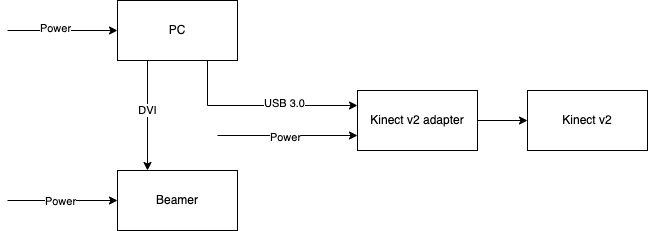
\includegraphics[width=0.9\textwidth]{img/cablesScheme.png}
	\caption*{Lo schema dei cavi}
\end{figure}

\begin{figure}[H]
	\centering
	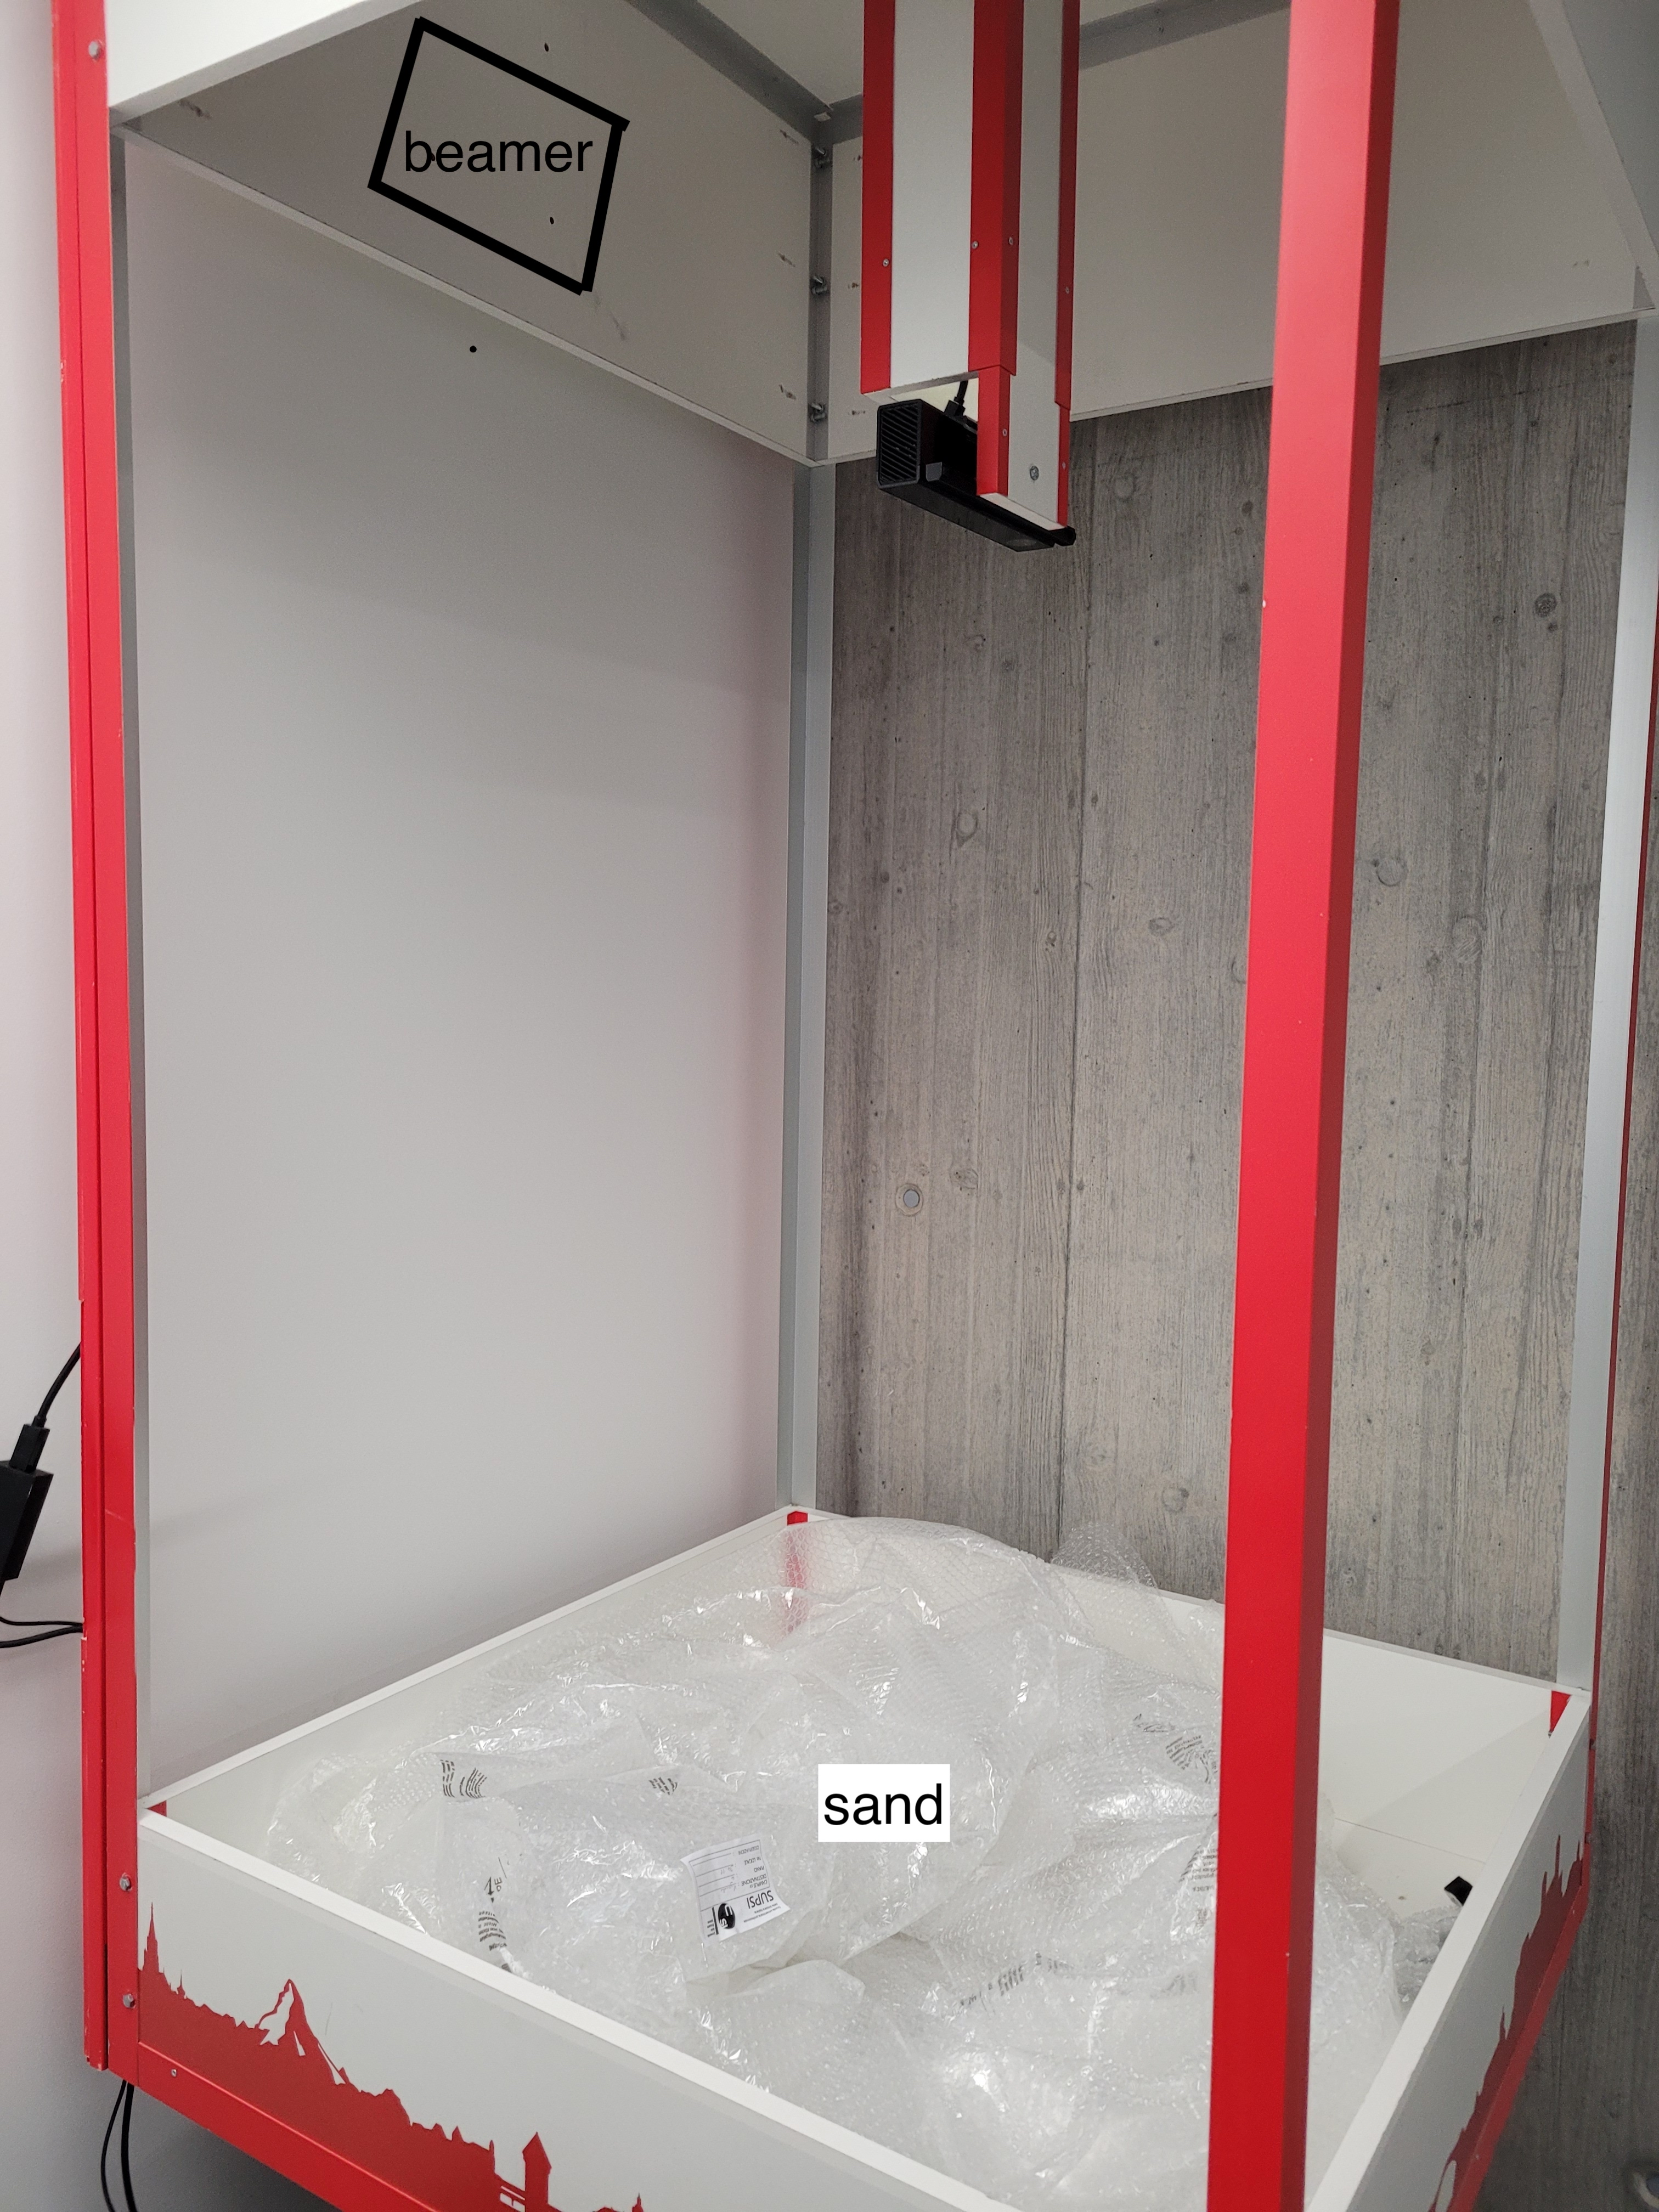
\includegraphics[width=0.85\textwidth]{img/sandbox.jpg}
	\caption*{La sandbox assemblata con il proiettore (1), il Kinect (2) e il suo adattatore (3), e il PC (4)}
\end{figure}


\subsection{Avvio}

ATTENZIONE: \textbf{NON} collegare il PC a internet per nessun motivo! Gli ultimi aggiornamenti
di Windows interferiscono con il funzionamento del sensore Kinect.\\

Avviare il PC premendo il tasto d'accensione e attendere l'avvio automatico del software. In caso il proiettore non dovesse avviarsi da solo, premere il relativo tasto d'accensione.\\
In caso di bisogno è possibile avviare il software manualmente cliccando sul collegamento
\texttt{Launch sandbox} sul Desktop.\\

Una volta aperto il software, le mucche dovrebbero iniziare a muoversi da sole sul terreno. Qualora non fosse il caso e
il terreno dovesse restare sempre beige, premere brevemente il tasto \texttt{RESET} sul lato anteriore del PC
e aspettare il riavvio del sistema.\\


\subsection{Spegnimento}

Premere brevemente il tasto di alimentazione del PC per arrestare normalmente il sistema e
attendere lo spegnimento automatico del proiettore. \textbf{NON} scollegarlo
dalla corrente fintanto che	il LED arancione lampeggia (raffreddamento in corso)!


\section{Utilizzo}

Il programma riconosce dinamicamente, grazie al sensore Kinect, i cambiamenti di altezza della sabbia
e adatta automaticamente l'immagine proiettata. Gli animali (mucche o pesci, a dipendenza del terreno
selezionato) camminano unicamente sulle superfici dov'è possibile, anch'essi adattandosi all'ambiente
che li circonda.

\subsection{Operazioni frequenti}

Cambiare terreno: F5 $\rightarrow$ F1/F2/F3 $\rightarrow$ F5

Regolare altezza: F5 $\rightarrow$ Spazio $\rightarrow$ U/J per la minima e I/K per la massima $\rightarrow$ F5

Regolare dimensioni immagine: F5 $\rightarrow$ Spazio $\rightarrow$ vedi sotto per i tasti $\rightarrow$ F5

\newpage
\subsection{Tasti utili}\label{sec:commands}

In modalità normale

\begin{tabular}{l l}
	ESC & esci                    \\
	P   & salva mesh              \\
	F5  & entra in modalità setup \\
	-   & mostra solo terreno     \\
\end{tabular}

In modalità setup

\begin{tabular}{l l}
	F1      & seleziona terreno 1 (montagne con mucche)        \\
	F2      & seleziona terreno 2 (lava)                       \\
	F3      & seleziona terreno 3 (pianure con pesci)          \\

	F5      & esci dalla modalità setup                        \\

	1/2/3/4 & seleziona angolo                                 \\
	5       & ridimensiona terreno                             \\
	6       & muovi terreno                                    \\

	W/A/S/D & sposta il terreno nella direzione corrispondente \\
	Shift   & movimento più lento                              \\

	Spazio  & attiva/disattiva anteprima                       \\

	9       & salva calibrazione su disco                      \\
	0       & carica calibrazione dal disco                    \\

	U/J     & aumenta/riduci l'altezza minima                  \\
	I/K     & aumenta/riduci l'altezza massima                 \\
\end{tabular}

\section{Problemi frequenti}

\subsection{L'immagine non corrisponde alla dimensione della sandbox}

In modalità setup, premere il tasto 0 per caricare l'ultima configurazione salvata e
Spazio per vedere un'anteprima. È possibile regolare l'immagine con i comandi descritti
al capitolo \ref{sec:commands}. Per uscire dalla modalità setup, premere nuovamente il tasto F5.\\

\subsection{L'applicazione si chiude improvvisamente}

Il terreno con le mucche (selezionato di default) è molto pesante e può fare crashare l'applicazione.
In caso dovesse succedere, in modalità setup è possibile selezionare con il tasto F3 un altro terreno simile
ma più leggero (pesci).

\subsection{L'immagine è sfocata o di cattiva qualità}

Provare a regolare il focus del proiettore con l'aiuto della ghiera sulla lampada. In caso non migliorasse, controllare
che il proiettore \textbf{non} sia in modalità 3D (menu $\rightarrow$ stereo $\rightarrow$ stereo mode).

\subsection{Non ci sono mucche e il terreno rimane sempre beige}

Premere brevemente il tasto \texttt{RESET} sul lato anteriore del PC e aspettare il riavvio.


\section{Codice sorgente}\label{sec:code}

Il codice sorgente dell'applicazione, assieme alle istruzioni per compilarla, si trova alla pagina \url{https://github.com/USI-Showroom/ARSandbox}.


\end{document}
